\documentclass[11pt]{article}
\usepackage{lmodern}
\usepackage[T1]{fontenc}

% ==============================================================================
% Packages — mirror the example explainer (intuitive_writeup.tex) so the voice,
% sectioning, and coloured callout boxes match the rest of the project's docs.
% ==============================================================================
\usepackage[margin=1in]{geometry}
\usepackage{amsmath, amssymb}
\usepackage{graphicx}
\usepackage{booktabs}
\usepackage{microtype}
\microtypesetup{expansion=false}
\usepackage{hyperref}
\usepackage{xcolor}
\usepackage{tikz}
\usepackage[most]{tcolorbox}
\usepackage{enumitem}
\usetikzlibrary{arrows.meta, positioning, decorations.pathreplacing,
                calc, shapes.geometric, patterns, fit, backgrounds}

\hypersetup{colorlinks=true, linkcolor=blue!50!black,
            urlcolor=blue!50!black, citecolor=blue!50!black}

% A blue "key numbers / tables" box and a yellow "primer / aside" box, exactly as
% the example uses, so a reader who has seen one project doc feels at home here.
\newtcolorbox{numbersbox}[1][]{
  colback=blue!5, colframe=blue!50!black, fonttitle=\bfseries,
  title={#1}, sharp corners, boxrule=0.6pt}

\newtcolorbox{primerbox}[1][]{
  colback=yellow!10, colframe=orange!70!black, fonttitle=\bfseries,
  title={#1}, sharp corners, boxrule=0.6pt}

% A green "rule we never break" box — the provenance / non-destructive invariants.
\newtcolorbox{rulebox}[1][]{
  colback=green!5, colframe=green!45!black, fonttitle=\bfseries,
  title={#1}, sharp corners, boxrule=0.6pt}

\newcommand{\code}[1]{\texttt{\small #1}}

\title{The temporal knowledge graph \& the date model\\[2pt]
       \large reconstructing structure, time, and provenance in the Solanus Casey archive}
\author{}
\date{}

\begin{document}
\maketitle

\begin{abstract}
\noindent
Fr.\ Solanus Casey's archive is 570 letters and 716 notebook pages, and it hides its own structure: a
single favor spills across a page break, a date is written once and then omitted for a dozen entries,
and the \emph{year} never appears in an entry at all --- it sits at the top of the page. This note
explains, from first principles, the three \code{step\_7} stages that recover that structure ---
\code{stitch\_notebooks} (cross-page continuation), \code{normalize\_dates} (the date model: split
month/day $+$ archival year, carry-forward, EDTF, bitemporal), and \code{build\_graph} (a RiC-O
temporal knowledge graph with link-prediction) --- and the two rules that run through all of them:
\emph{every fact cites the exact handwritten region it came from}, and \emph{nothing destructive or
billed happens without an explicit, gated opt-in}.
\end{abstract}

\tableofcontents
\bigskip

% ==============================================================================
\section{TL;DR}
% ==============================================================================

\begin{itemize}[leftmargin=1.4em]
  \item \textbf{The corpus hides its structure.} One favor is split across "Page 1 Cont."; a date is
        written once and omitted thereafter; the year lives in the page header (\code{archv\_date}),
        never in the entry. We must \emph{reconstruct} the whole thought and its real date before any
        search or graph work.
  \item \textbf{Three stages, in dependency order, each a brand-new artifact} (we never edit
        \code{documents.json} / \code{notebooks.json}):
        \begin{enumerate}[leftmargin=1.6em, label=\arabic*.]
          \item \code{stitch\_notebooks} joins split entries into one \textbf{logical entry} while
                keeping each fragment's exact region box. $\to$ \code{data/stitched\_notebooks.json}
          \item \code{normalize\_dates} assembles \code{month/day} $+$ \code{archival year} $+$
                \textbf{carry-forward} into a canonical \textbf{EDTF} date, and captures
                \textbf{two} dates per favor (enrolled vs.\ reported). $\to$ \code{data/dates.json}
          \item \code{build\_graph} builds a \textbf{networkx} graph aligned to \textbf{RiC-O}, with
                \textbf{provenance} and \textbf{EDTF valid-time on every edge}, exports
                \code{graph.json} (viz) $+$ \code{graph.ttl} (RDF), and ships a \textbf{KGE
                link-prediction} scaffold that \emph{proposes} edges into a review queue.
        \end{enumerate}
  \item \textbf{Two unbreakable rules.} (1)~\emph{Provenance-first}: every fact points back to
        \code{doc\_id + rid + page + vertices} so the app deep-zooms to the exact ink.
        (2)~\emph{Non-destructive, David-only gold}: rule paths are free and deterministic; every LLM
        step is gated off by default and cost-logged; suggested links go to a review queue, never the
        graph.
\end{itemize}

\begin{rulebox}[The receipts rule]
An archive that cannot show its receipts is just a rumor with footnotes. So no assertion in this
pipeline floats free: each one carries the region id(s) it was read from, and the web app turns those
into an IIIF deep-zoom straight to the handwriting. This single constraint shapes every data structure
below.
\end{rulebox}

% ==============================================================================
\section{Why a graph, and why a date model?}
% ==============================================================================

The retrieval layer (embeddings over chunks) is excellent at one question: \emph{``which passages look
similar to what I typed?''} But an archivist asks a different \emph{kind} of question --- relational
and aggregate:

\begin{itemize}[leftmargin=1.4em]
  \item \emph{Whom did Solanus write to in 1896, and from where?}
  \item \emph{Which favors reported a cure, and which conditions recur across the Casey family?}
  \item \emph{Which notebook entries continue onto the next page?}
\end{itemize}

Those are graph questions: they are about \emph{edges} (wrote-to, has-condition, continues-on) and
\emph{time} (in 1896, as-of 1933). A knowledge graph is the natural home. And every one of those
questions has a \emph{when} attached, which is why the date model has to come first: an edge without a
trustworthy date is half an edge.

% ==============================================================================
\section{Stage 1 --- \texttt{stitch\_notebooks}: reconstruct the logical entry}
% ==============================================================================

\subsection{The problem, concretely}

The notebooks are a \emph{running register}. When Solanus ran out of room he simply kept writing on the
next page, and the archive labels the spill-over literally. Here is a real page from the corpus
(\code{Volume\_3\_\_p002}, pdf page~3), whose first entry is labelled \code{"Page 1 Cont."}:

\begin{quote}\small
\textbf{Page 1 Cont.} --- ``Mary Briggi - joined her brother V. today -- been drinking for five years
-- Very careless about Church etc. Dec.\ 14th re- ports very hopeful that his drinking\ldots''
\end{quote}

\noindent``Page 1 Cont.'' means \emph{this is still page 1, continued}: the thought that ran off the
bottom of the previous page resumes here. If we hand those raw halves to retrieval, the reader --- and
the embedding model --- sees a half-sentence with no date and no context. So before anything else, we
rebuild the \textbf{logical entry}: the complete unit of meaning, possibly made of several raw
fragments.

\subsection{The walk, and the cheap signals}

We consider joining only the \emph{tail of one page} to the \emph{head of the very next page} --- the
single place a physical page-break can split a thought. The decision uses transparent, auditable cues:

\begin{numbersbox}[The continuation signals (additive, not a black box)]
\centering\small
\begin{tabular}{lll}
\toprule
signal & what it detects & weight \\
\midrule
\code{page\_label =\textasciitilde\ /cont/i} & next page literally says ``\ldots\ Cont.'' & $+0.55$ \\
numbered chain & ``Page N'' $\to$ ``Page N Cont.'', N matches & $+0.25$ \\
truncated tail & prev entry ends mid-clause (no \code{.\,!\,?\,…}\ / dash; or \code{"As-"}) & $+0.20$ \\
orphan head & next entry opens lower-case or on a connective & $+0.15$ \\
\bottomrule
\end{tabular}
\end{numbersbox}

\noindent A page-break with a confidence $\ge$ threshold (default $0.55$, so an explicit ``Cont.''
label alone clears the bar) is a candidate join. Grouping into registers is itself non-trivial: the
OCR'd notebook header is wildly inconsistent (\code{"FR. SOLANUS, NOTEBOOK NO. 5."},
\code{"FR. SOLNAUS, NOTEBOOK NO. S."}, \ldots\ all the \emph{same} book), so we group on
\code{section} $+$ a \emph{normalized notebook number} rather than the raw string --- otherwise one
book shatters into 50+ micro-registers and real joins vanish (we measured 154 adjacent page-pairs
broken this way).

\subsection{The one distinction that prevents disaster}

\begin{rulebox}[Page-level continuation $\neq$ entry-level continuation]
``Page N Cont.'' tells us the \emph{register} continues onto the next page. It does \textbf{not} tell
us the last favor on page N is the \emph{same favor} as the first favor on the Cont.\ page --- usually
the Cont.\ page just lists the \emph{next person}. Fusing those would be a \textbf{false merge}: two
unrelated people's stories welded into one logical entry.

\medskip
So we \textbf{fuse two entries} only when the \emph{thought itself} is split (tail truncated
\emph{or} head orphaned) $\Rightarrow$ \code{continues\_on}/\code{continued\_from} edges. When the
label says Cont.\ but both halves are complete favors, we keep a \emph{page-level}
\code{page\_continues\_on} edge (the register flows on) and \textbf{leave the entries distinct}.
\end{rulebox}

\noindent This is the whole pipeline's bias in one line: \emph{we would rather under-stitch (a missing
link David can recover later via link-prediction) than over-stitch (a corrupted logical entry).}

\begin{center}
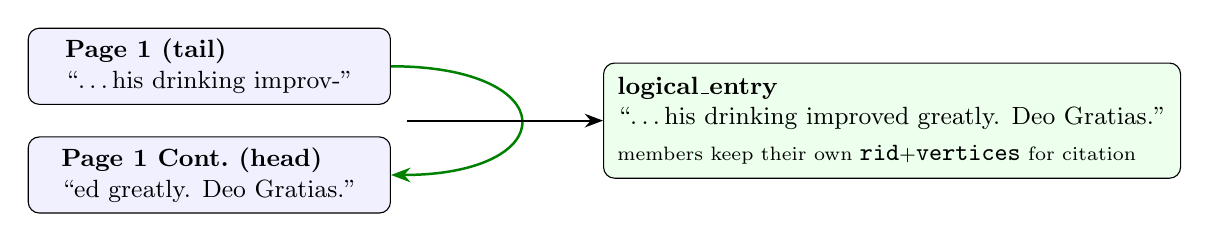
\begin{tikzpicture}[font=\small, node distance=4mm,
   frag/.style={draw, rounded corners, fill=blue!6, minimum width=4.6cm, align=left, inner sep=4pt},
   le/.style={draw, rounded corners, fill=green!7, minimum width=5.0cm, align=left, inner sep=5pt}]
  % page A tail
  \node[frag] (a) {\textbf{Page 1 (tail)}\\ ``\ldots his drinking improv-''};
  % page B head, truncated/orphan -> join
  \node[frag, below=of a] (b) {\textbf{Page 1 Cont.\ (head)}\\ ``ed greatly. Deo Gratias.''};
  % the join arrow
  \draw[-{Stealth[]}, line width=0.9pt, green!50!black]
        (a.east) .. controls +(2.2,0) and +(2.2,0) .. (b.east)
        node[midway, right=1.6cm, green!45!black, align=left]
        {tail truncated\\$+$ head orphan\\$\Rightarrow$ \textbf{fuse}};
  % logical entry
  \node[le, right=5.0cm of $(a)!0.5!(b)$] (L)
       {\textbf{logical\_entry}\\ ``\ldots his drinking improved greatly. Deo Gratias.''\\[2pt]
        \scriptsize members keep their own \code{rid}+\code{vertices} for citation};
  \draw[-{Stealth[]}, thick] ([xshift=2mm]a.east|-L.west) -- (L.west);
\end{tikzpicture}
\end{center}

\subsection{What it writes}

\code{data/stitched\_notebooks.json}: \code{logical\_entries} (the whole-favor unit retrieval should
embed), \code{relations} (the KG edges), and an \code{ambiguous\_joins} review queue. Every member
fragment retains \code{rid} $+$ \code{vertices} $+$ \code{min\_conf}, so a citation still deep-zooms to
the precise box even though retrieval now sees the whole entry. That is the ``keep both'' rule.

\begin{primerbox}[The gated multimodal step (no call is made)]
\code{confirm\_join\_with\_vision(\ldots)} would show a vision model the \emph{bottom of page A and the
top of page B} and ask whether the thought continues --- the 2026 archival-continuation approach,
because layout cues (indentation, a bracket, a ditto mark) survive in the image but not in OCR text.
It is \textbf{gated off}; \code{run()} makes zero calls. Wiring it is a one-place TODO, and the call
would be cost-logged via \code{lib.providers.llm} $\to$ \code{lib.costlog}.
\end{primerbox}

% ==============================================================================
\section{Stage 2 --- \texttt{normalize\_dates}: the date model}
% ==============================================================================

\subsection{The problem, concretely}

An entry usually carries only a month and day (``Mar.\ 30''), sometimes only a bare day (``22''). The
\textbf{year almost never appears in the entry}; it lives once, at the top of the page, in
\code{archv\_date} (e.g.\ ``1923, November''). And the dates are gloriously human: circa
(``c.\ 1929''), ranges (``c.\ 1897 to 1904''), feast days, and --- crucially for the favors timeline
--- \emph{two} dates inside one entry.

\subsection{Four moves}

\paragraph{(1) Hierarchical assembly.} Year from the page; month/day from the entry; combine.

\paragraph{(2) Carry-forward.} Exactly how a human reads a register: a bare ``the 17th'' means ``the
17th of \emph{whatever month we're in}''. A missing month is inherited from the previous entry; a
missing year from the page (or the last year resolved on it). Each inference is a small, transparent
\textbf{confidence} debit --- $1.0$ means ``fully read,'' lower means ``partly inferred.''

\paragraph{(3) The year-boundary trick.} A single page often straddles New Year, and the archival
field records it as month/year \emph{pairs}. A real example:
\[
\code{archv\_date} = \texttt{"1923, December\ \ 1924, January"}.
\]
A naïve ``first year wins'' rule dates \emph{every} January entry on that page to \textbf{1923} --- a
guaranteed one-year error. Instead we build a small \textbf{month\,$\to$\,year} map from the field
($\text{Dec}\!\to\!1923,\ \text{Jan}\!\to\!1924$) and pick the year matching the entry's resolved
month. A January entry correctly becomes \textbf{1924}. The year-boundary page goes from a systematic
bug to a correctly \emph{split} timeline.

\paragraph{(4) Bitemporal scan.} Favor entries record an \textbf{enrollment} date and a later
\textbf{report/outcome} date. A real example (\code{Volume\_3\_\_p002::doc\_1.src\_content.10}):
\begin{quote}\small
``Mrs.\ Catheline M.\ Sawler \textbf{Enrolled May 3rd 1923} --- given 3 days to live with pneumonia
\ldots\ \textbf{report - Recovered} completely\ldots''
\end{quote}
We scan the body just after the cue words (\code{enroll*}, \code{report*}/\code{recovered}) and date
each separately, so the enrollment and the outcome carry their \emph{own} valid-times instead of one
blurred date. \emph{That} is what makes a real favors timeline possible.

\subsection{Why EDTF}

Archival dates are fuzzy, and EDTF (Extended Date/Time Format, ISO 8601-2, Library of Congress) lets us
store the fuzziness \emph{as data} instead of discarding it or faking precision. We always encode at
the precision we actually have --- no more:

\begin{numbersbox}[EDTF, by example (from the Solanus corpus)]
\centering\small
\begin{tabular}{ll p{6.2cm}}
\toprule
corpus date & EDTF & what the notation means \\
\midrule
Aug.\ 23rd, 1896          & \code{1896-08-23}      & full date \\
October 1933, day unknown & \code{1933-10-XX}      & \code{X} = a known-unknown digit \\
(only a year survives)    & \code{1929}            & ``some time in 1929'' \\
c.\ 1945                  & \code{1945\textasciitilde} & \code{\textasciitilde} = approximate / circa \\
Feb--Oct 1940             & \code{1940-02/1940-10} & \code{A/B} = a closed range \\
\bottomrule
\end{tabular}
\end{numbersbox}

\subsection{Two code paths}

A \textbf{pure-Python rule path} (\code{reconstruct\_record}) does the whole job --- free,
deterministic, no key, no model download --- and is what \code{run()} executes by default, so the
temporal layer is reproducible and costs nothing. A real but \textbf{gated} \textbf{LLM normalizer}
(\code{llm\_normalize\_date}) handles the genuinely hard strings (feast days, garbled OCR, prose
dates); it is \textbf{off} unless \code{use\_llm=True}, capped by \code{llm\_max}, only escalates the
\emph{lowest-confidence} records, and is cost-logged on every call.

\medskip
\noindent\textbf{Output:} \code{data/dates.json}, keyed by record id, each row carrying \code{raw} +
\code{edtf} + \code{precision} (\code{unknown\,|\,year\,|\,month\,|\,day\,|\,range}) +
\code{confidence} + \code{circa} + \code{method} + the bitemporal \code{enrolled}/\code{reported}
pair. The raw string sits next to the EDTF value, so every reconstruction is auditable.

% ==============================================================================
\section{Stage 3 --- \texttt{build\_graph}: the RiC-O temporal knowledge graph}
% ==============================================================================

\subsection{One graph, two exports}

We build the truth once in \textbf{networkx} (a \code{MultiDiGraph} --- \emph{multi} because two
entities can be tied by more than one relation; \emph{di} because most relations are directed), then
project the same facts into RDF:

\begin{itemize}[leftmargin=1.4em]
  \item \code{data/graph.json} --- a node/edge list for the web visualization (D3 / Cytoscape).
  \item \code{data/graph.ttl} --- \textbf{RiC-O} RDF (Turtle), so the archive is interoperable Linked
        Data, not a one-off blob. RiC-O (\emph{Records in Contexts}, the ICA's ontology) is proven on
        scholarly correspondence. Where RiC-O has a tidy property we use it; where it doesn't, we use a
        clearly project-namespaced predicate so nothing masquerades as standard vocabulary.
\end{itemize}

Both exporters read the \emph{same} edge-verb table (\code{EDGE\_KINDS}), so the JSON and the TTL can
never drift apart. The verbs: \code{WROTE\_TO}, \code{LOCATED\_AT}, \code{MEMBER\_OF}, \code{FAMILY},
\code{ENROLLED}, \code{PETITIONED\_FOR}, \code{HAS\_CONDITION}, \code{HAS\_OUTCOME},
\code{MENTIONED\_IN}, \code{CONTINUES\_ON}. Records become RiC-O \code{Record}/\code{RecordPart};
people/orgs/places become \code{Person}/\code{CorporateBody}/\code{Place}; a favor becomes an
\code{Activity} (an enrollment/report is best modeled as an event).

\subsection{Where the edges come from --- cheapest and most reliable first}

\begin{numbersbox}[Edge sources, ranked by trust]
\centering\small
\begin{tabular}{lll}
\toprule
edge & source & \code{method} tag \\
\midrule
\code{WROTE\_TO}, \code{LOCATED\_AT} & letters' separated recipient/sender/location fields & \code{source} \\
\code{MENTIONED\_IN} (gold)          & \code{entry.linked} (David's curated connection graph) & \code{gold\_link} \\
\code{CONTINUES\_ON}                 & \code{stitched\_notebooks.json} (else \code{/cont/} fallback) & \code{stitch} \\
\code{ENROLLED}/\code{HAS\_OUTCOME}  & \code{normalize\_dates} bitemporal $+$ lexical favor cues & \code{lexical\_cue} \\
\code{HAS\_CONDITION}                & conservative condition cues in entry text & \code{lexical\_cue} \\
\bottomrule
\end{tabular}
\end{numbersbox}

\noindent Correspondence is a \emph{free head-start}: recipient, sender, and location are already
separated fields per letter. The real letter \code{Volume\_1\_\_p001} (``Very Rev.\ Bonaventure
Frey'', ``Aug.\ 23rd, 1896'') yields, in one step:
\[
\underbrace{\text{Father Solanus Casey}}_{\text{person}}
\ \xrightarrow{\ \code{WROTE\_TO}\ }\
\underbrace{\text{Very Rev.\ Bonaventure Frey}}_{\text{person}},
\quad
\code{valid\_time}=\texttt{1896-08-23},\ \ \code{rid}=\texttt{doc\_1.src\_recipient.0}.
\]
The lexical favor cues (tagged \code{lexical\_cue}) are deliberately shallow --- they exist so the
favors backbone is \emph{present} before the proper LLM extractor (\code{extract\_entities}) lands and
supersedes them. We would rather miss an edge than assert a wrong one in an archive.

\subsection{Two ideas that make the graph trustworthy for an archive}

\paragraph{Provenance on every edge (via reification).} ``Solanus wrote to X \emph{in 1896}, \emph{as
evidenced by region} \code{doc\_5.src\_recipient.0}'' is a statement \emph{about} a statement ---
provenance and time are metadata \emph{on the edge}, and an RDF edge cannot carry attributes directly.
So we \textbf{reify}: mint a blank node for the statement and hang the rids off it with PROV-O
\code{prov:wasDerivedFrom}, and the valid-time as a \code{rico:date} EDTF literal. The receipts stay
attached.

\begin{center}
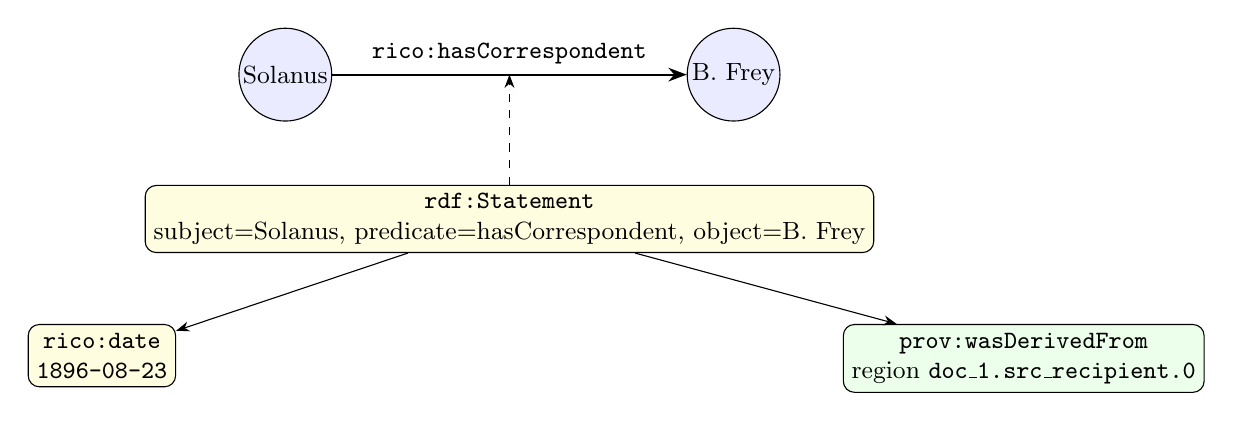
\begin{tikzpicture}[font=\small,
  ent/.style={draw, circle, fill=blue!8, minimum size=1.0cm, align=center, inner sep=1pt},
  stmt/.style={draw, rounded corners, fill=yellow!12, align=center, inner sep=3pt},
  reg/.style={draw, rounded corners, fill=green!8, align=center, inner sep=3pt}]
  \node[ent] (s) {Solanus};
  \node[ent, right=4.5cm of s] (o) {B.\ Frey};
  \draw[-{Stealth[]}, thick] (s) -- node[above]{\code{rico:hasCorrespondent}} (o);
  % reified statement hanging below the edge
  \node[stmt, below=1.4cm of $(s)!0.5!(o)$] (st)
       {\code{rdf:Statement}\\ subject=Solanus, predicate=hasCorrespondent, object=B.\ Frey};
  \draw[-{Stealth[]}, dashed] (st.north) -- ($(s)!0.5!(o)$);
  \node[stmt, below left=0.9cm and -0.4cm of st] (t) {\code{rico:date}\\ \texttt{1896-08-23}};
  \node[reg, below right=0.9cm and -0.4cm of st] (r)
       {\code{prov:wasDerivedFrom}\\ region \texttt{doc\_1.src\_recipient.0}};
  \draw[-{Stealth[]}] (st) -- (t);
  \draw[-{Stealth[]}] (st) -- (r);
\end{tikzpicture}
\end{center}

\paragraph{Valid-time in EDTF on every edge.} Because each edge carries a \emph{when}, the viz can
later do ``as-of 1933'' point-in-time views --- show the network exactly as the record stood at a
chosen moment.

\subsection{Link prediction: a review queue, never an edit}

Knowledge graphs are always \emph{incomplete}: a continuation wasn't stitched, two name variants
weren't merged, a family tie is implied but never written. A \textbf{KG-embedding} model learns a
vector $\mathbf{e}_h, \mathbf{e}_t$ per entity and $\mathbf{r}$ per relation so a \emph{true} triple
$(h, r, t)$ scores high. DistMult, for instance, scores a triple by a simple three-way inner product,
\[
\mathrm{score}(h, r, t) \;=\; \langle \mathbf{e}_h,\ \mathbf{r},\ \mathbf{e}_t \rangle
\;=\; \sum_{i} e_{h,i}\, r_i\, e_{t,i},
\]
trained so observed triples outscore randomly corrupted ones. You then score \emph{un-asserted}
triples and rank the most plausible missing edges. The stage ships this as a deliberate
\textbf{scaffold}:

\begin{itemize}[leftmargin=1.4em]
  \item \code{train=False} (default) writes an empty-but-valid \code{data/graph\_suggestions.json}, so
        the review UI always has something well-formed to read.
  \item \code{train=True} runs a tiny pure-NumPy DistMult \emph{smoke trainer} (CPU, free) so the
        control flow is real and runnable, with type constraints so it only proposes \emph{type-sane}
        edges (a place can't ``continue onto'' a condition).
  \item The production path is a clearly-marked \textbf{TODO} that plugs in \textbf{pykeen} (pulls
        torch --- not yet in the venv).
\end{itemize}

\begin{rulebox}[Suggestions are not assertions]
Every proposed edge lands in \code{graph\_suggestions.json} with \code{status: "proposed"} and the
evidence rids that explain \emph{why} it was suggested. David confirms. \textbf{Gold is David-only;
nothing merges into \code{graph.json}/\code{graph.ttl} automatically.} This turns ``missing
connections'' from a dead end into a finite review queue.
\end{rulebox}

% ==============================================================================
\section{How to run it}
% ==============================================================================

\begin{numbersbox}[Commands (all FREE by default; nothing is billed)]
\small
\begin{verbatim}
source pipeline_v3/step_7/venv/bin/activate
pip install networkx rdflib          # build_graph's two (lazy) deps

# dependency order:
python stages/stitch_notebooks.py    # -> data/stitched_notebooks.json
python stages/normalize_dates.py     # -> data/dates.json
python stages/build_graph.py         # -> data/graph.json + graph.ttl + suggestions

# smoke tests / inspection:
python stages/stitch_notebooks.py --limit-groups 3
python stages/normalize_dates.py  --limit 50
python stages/normalize_dates.py  --print "Volume_3__p002::doc_1.src_content.10"
python stages/build_graph.py      --kge --top-k 50    # local NumPy KGE smoke
\end{verbatim}
\end{numbersbox}

\noindent\textbf{Order matters, but absence never crashes.} \code{build\_graph} \emph{prefers}
\code{dates.json} and \code{stitched\_notebooks.json}, yet degrades gracefully without them (its own
conservative date parser; a \code{/cont/} heuristic; a record-only graph if \code{entities.json} is
still a stub). Running the stages in order simply makes the graph richer and more accurate. To enable
the paid steps \emph{only when David says go}: \code{normalize\_dates.run(use\_llm=True,
llm\_max=<budget>)} and wire the \code{confirm\_join\_with\_vision} TODO --- both auto-cost-logged.

% ==============================================================================
\section{Caveats}
% ==============================================================================

\begin{itemize}[leftmargin=1.4em]
  \item \textbf{Heavy deps deferred.} \code{build\_graph} needs \code{networkx} + \code{rdflib}
        (imported lazily, so importing the module never explodes); production KGE needs
        \code{pykeen}/torch. None are installed yet --- the stage stays inspectable and the smoke
        trainer runs without them.
  \item \textbf{Lexical favor cues are shallow} (substring matches, tagged \code{lexical\_cue}); they
        seed the favors backbone before the real \code{extract\_entities} LLM stage supersedes them.
  \item \textbf{The rule date parser is conservative} on purpose; the dedicated normalizer is the
        source of truth, and \code{build\_graph.to\_edtf} is only a fallback so the graph has
        \emph{some} valid-time before \code{dates.json} exists.
  \item \textbf{We under-stitch deliberately.} A missed join is recoverable later (the KGE review
        queue); a false merge corrupts a logical entry. The thresholds encode that bias.
  \item \textbf{Prices in \code{config.py} are placeholders} until verified against each provider's
        page --- but nothing is billed until a gate is flipped.
\end{itemize}

% ==============================================================================
\section{Sources}
% ==============================================================================

\begin{itemize}[leftmargin=1.4em]
  \item \textbf{EDTF (ISO 8601-2)} --- Library of Congress:
        \url{https://www.loc.gov/standards/datetime/};
        validator: \url{https://digital2.library.unt.edu/edtf/}.
  \item \textbf{RiC-O (Records in Contexts Ontology)} --- International Council on Archives:
        \url{https://www.ica.org/standards/RiC/ontology}.
  \item \textbf{PROV-O (Provenance Ontology)} --- W3C: \url{https://www.w3.org/TR/prov-o/}.
  \item \textbf{Cross-page continuation via multimodal LLMs} (historical registers):
        \url{https://arxiv.org/pdf/2512.19675}.
  \item \textbf{KG embeddings / link prediction} --- completion review:
        \url{https://www.mdpi.com/2078-2489/13/8/396}; \textbf{pykeen}:
        \url{https://github.com/pykeen/pykeen}.
  \item \textbf{networkx} \url{https://networkx.org/} \quad \textbf{rdflib}
        \url{https://rdflib.readthedocs.io/}.
  \item Project plan: \code{pipeline\_v3/step\_7/RESEARCH\_PLAN.md} (PART~A: A1 continuation, A2 dates;
        PART~C: temporal KG + KGE).
\end{itemize}

% ------------------------------------------------------------------------------
% BUILD NOTE (do not compile here): keep ALL aux files in build/ via
%   latexmk -pdf -outdir=build graph_and_dates.tex
% so only graph_and_dates.tex and build/graph_and_dates.pdf result. The optional
% latexmkrc beside this file sets that as the default $out_dir.
% ------------------------------------------------------------------------------

\end{document}
